\documentclass{article}
\usepackage{tikz}
\usetikzlibrary{positioning}

\begin{document}

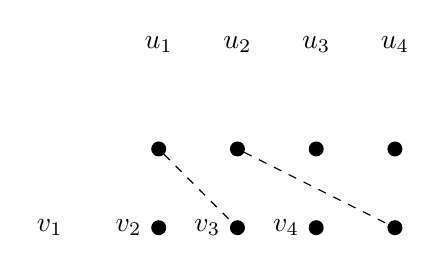
\begin{tikzpicture}[node distance=1cm]
    \node (u1) [circle, draw, fill=black, inner sep=0pt, minimum size=5pt] at (0,0) {};
    \node (u2) [circle, draw, fill=black, inner sep=0pt, minimum size=5pt] at (1,0) {};
    \node (u3) [circle, draw, fill=black, inner sep=0pt, minimum size=5pt] at (2,0) {};
    \node (u4) [circle, draw, fill=black, inner sep=0pt, minimum size=5pt] at (3,0) {};
    
    \node (v1) [circle, draw, fill=black, inner sep=0pt, minimum size=5pt] at (0,-1) {};
    \node (v2) [circle, draw, fill=black, inner sep=0pt, minimum size=5pt] at (1,-1) {};
    \node (v3) [circle, draw, fill=black, inner sep=0pt, minimum size=5pt] at (2,-1) {};
    \node (v4) [circle, draw, fill=black, inner sep=0pt, minimum size=5pt] at (3,-1) {};
    
    \draw[dashed] (u1) -- (v2);
    \draw[dashed] (u2) -- (v4);
    
    \node[above=of u1] {$u_1$};
    \node[above=of u2] {$u_2$};
    \node[above=of u3] {$u_3$};
    \node[above=of u4] {$u_4$};
    
    \node[left=of v1] {$v_1$};
    \node[left=of v2] {$v_2$};
    \node[left=of v3] {$v_3$};
    \node[left=of v4] {$v_4$};
\end{tikzpicture}

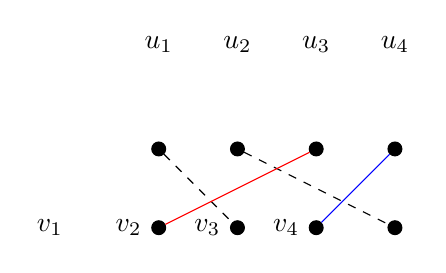
\begin{tikzpicture}[node distance=1cm]
    \node (u1) [circle, draw, fill=black, inner sep=0pt, minimum size=5pt] at (0,0) {};
    \node (u2) [circle, draw, fill=black, inner sep=0pt, minimum size=5pt] at (1,0) {};
    \node (u3) [circle, draw, fill=black, inner sep=0pt, minimum size=5pt] at (2,0) {};
    \node (u4) [circle, draw, fill=black, inner sep=0pt, minimum size=5pt] at (3,0) {};
    
    \node (v1) [circle, draw, fill=black, inner sep=0pt, minimum size=5pt] at (0,-1) {};
    \node (v2) [circle, draw, fill=black, inner sep=0pt, minimum size=5pt] at (1,-1) {};
    \node (v3) [circle, draw, fill=black, inner sep=0pt, minimum size=5pt] at (2,-1) {};
    \node (v4) [circle, draw, fill=black, inner sep=0pt, minimum size=5pt] at (3,-1) {};
    
    \draw[dashed] (u1) -- (v2);
    \draw[dashed] (u2) -- (v4);
    \draw[red] (u3) -- (v1);
    \draw[blue] (u4) -- (v3);
    
    \node[above=of u1] {$u_1$};
    \node[above=of u2] {$u_2$};
    \node[above=of u3] {$u_3$};
    \node[above=of u4] {$u_4$};
    
    \node[left=of v1] {$v_1$};
    \node[left=of v2] {$v_2$};
    \node[left=of v3] {$v_3$};
    \node[left=of v4] {$v_4$};
\end{tikzpicture}

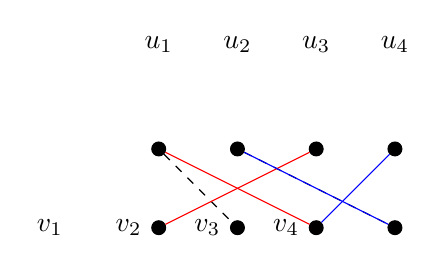
\begin{tikzpicture}[node distance=1cm]
    \node (u1) [circle, draw, fill=black, inner sep=0pt, minimum size=5pt] at (0,0) {};
    \node (u2) [circle, draw, fill=black, inner sep=0pt, minimum size=5pt] at (1,0) {};
    \node (u3) [circle, draw, fill=black, inner sep=0pt, minimum size=5pt] at (2,0) {};
    \node (u4) [circle, draw, fill=black, inner sep=0pt, minimum size=5pt] at (3,0) {};
    
    \node (v1) [circle, draw, fill=black, inner sep=0pt, minimum size=5pt] at (0,-1) {};
    \node (v2) [circle, draw, fill=black, inner sep=0pt, minimum size=5pt] at (1,-1) {};
    \node (v3) [circle, draw, fill=black, inner sep=0pt, minimum size=5pt] at (2,-1) {};
    \node (v4) [circle, draw, fill=black, inner sep=0pt, minimum size=5pt] at (3,-1) {};
    
    \draw[dashed] (u1) -- (v2);
    \draw[dashed] (u2) -- (v4);
    \draw[red] (u3) -- (v1);
    \draw[blue] (u4) -- (v3);
    \draw[red] (u1) -- (v3);
    \draw[blue] (u2) -- (v4);
    
    \node[above=of u1] {$u_1$};
    \node[above=of u2] {$u_2$};
    \node[above=of u3] {$u_3$};
    \node[above=of u4] {$u_4$};
    
    \node[left=of v1] {$v_1$};
    \node[left=of v2] {$v_2$};
    \node[left=of v3] {$v_3$};
    \node[left=of v4] {$v_4$};
\end{tikzpicture}

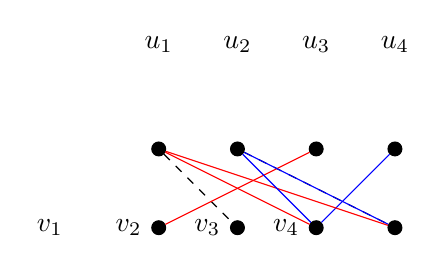
\begin{tikzpicture}[node distance=1cm]
    \node (u1) [circle, draw, fill=black, inner sep=0pt, minimum size=5pt] at (0,0) {};
    \node (u2) [circle, draw, fill=black, inner sep=0pt, minimum size=5pt] at (1,0) {};
    \node (u3) [circle, draw, fill=black, inner sep=0pt, minimum size=5pt] at (2,0) {};
    \node (u4) [circle, draw, fill=black, inner sep=0pt, minimum size=5pt] at (3,0) {};
    
    \node (v1) [circle, draw, fill=black, inner sep=0pt, minimum size=5pt] at (0,-1) {};
    \node (v2) [circle, draw, fill=black, inner sep=0pt, minimum size=5pt] at (1,-1) {};
    \node (v3) [circle, draw, fill=black, inner sep=0pt, minimum size=5pt] at (2,-1) {};
    \node (v4) [circle, draw, fill=black, inner sep=0pt, minimum size=5pt] at (3,-1) {};
    
    \draw[dashed] (u1) -- (v2);
    \draw[dashed] (u2) -- (v4);
    \draw[red] (u3) -- (v1);
    \draw[blue] (u4) -- (v3);
    \draw[red] (u1) -- (v3);
    \draw[blue] (u2) -- (v4);
    \draw[red] (u1) -- (v4);
    \draw[blue] (u2) -- (v3);
    
    \node[above=of u1] {$u_1$};
    \node[above=of u2] {$u_2$};
    \node[above=of u3] {$u_3$};
    \node[above=of u4] {$u_4$};
    
    \node[left=of v1] {$v_1$};
    \node[left=of v2] {$v_2$};
    \node[left=of v3] {$v_3$};
    \node[left=of v4] {$v_4$};
\end{tikzpicture}

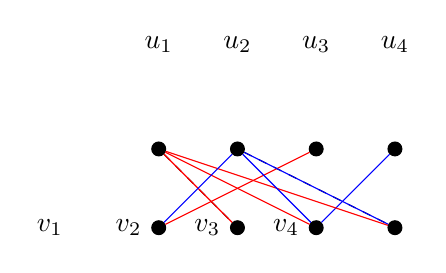
\begin{tikzpicture}[node distance=1cm]
    \node (u1) [circle, draw, fill=black, inner sep=0pt, minimum size=5pt] at (0,0) {};
    \node (u2) [circle, draw, fill=black, inner sep=0pt, minimum size=5pt] at (1,0) {};
    \node (u3) [circle, draw, fill=black, inner sep=0pt, minimum size=5pt] at (2,0) {};
    \node (u4) [circle, draw, fill=black, inner sep=0pt, minimum size=5pt] at (3,0) {};
    
    \node (v1) [circle, draw, fill=black, inner sep=0pt, minimum size=5pt] at (0,-1) {};
    \node (v2) [circle, draw, fill=black, inner sep=0pt, minimum size=5pt] at (1,-1) {};
    \node (v3) [circle, draw, fill=black, inner sep=0pt, minimum size=5pt] at (2,-1) {};
    \node (v4) [circle, draw, fill=black, inner sep=0pt, minimum size=5pt] at (3,-1) {};
    
    \draw[dashed] (u1) -- (v2);
    \draw[dashed] (u2) -- (v4);
    \draw[red] (u3) -- (v1);
    \draw[blue] (u4) -- (v3);
    \draw[red] (u1) -- (v3);
    \draw[blue] (u2) -- (v4);
    \draw[red] (u1) -- (v4);
    \draw[blue] (u2) -- (v3);
    \draw[red] (u1) -- (v2);
    \draw[blue] (u2) -- (v1);
    
    \node[above=of u1] {$u_1$};
    \node[above=of u2] {$u_2$};
    \node[above=of u3] {$u_3$};
    \node[above=of u4] {$u_4$};
    
    \node[left=of v1] {$v_1$};
    \node[left=of v2] {$v_2$};
    \node[left=of v3] {$v_3$};
    \node[left=of v4] {$v_4$};
\end{tikzpicture}

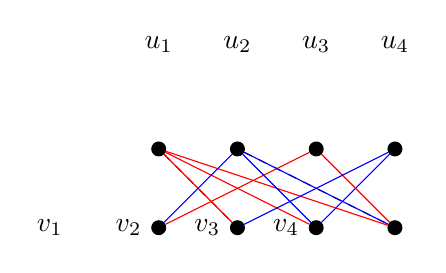
\begin{tikzpicture}[node distance=1cm]
    \node (u1) [circle, draw, fill=black, inner sep=0pt, minimum size=5pt] at (0,0) {};
    \node (u2) [circle, draw, fill=black, inner sep=0pt, minimum size=5pt] at (1,0) {};
    \node (u3) [circle, draw, fill=black, inner sep=0pt, minimum size=5pt] at (2,0) {};
    \node (u4) [circle, draw, fill=black, inner sep=0pt, minimum size=5pt] at (3,0) {};
    
    \node (v1) [circle, draw, fill=black, inner sep=0pt, minimum size=5pt] at (0,-1) {};
    \node (v2) [circle, draw, fill=black, inner sep=0pt, minimum size=5pt] at (1,-1) {};
    \node (v3) [circle, draw, fill=black, inner sep=0pt, minimum size=5pt] at (2,-1) {};
    \node (v4) [circle, draw, fill=black, inner sep=0pt, minimum size=5pt] at (3,-1) {};
    
    \draw[dashed] (u1) -- (v2);
    \draw[dashed] (u2) -- (v4);
    \draw[red] (u3) -- (v1);
    \draw[blue] (u4) -- (v3);
    \draw[red] (u1) -- (v3);
    \draw[blue] (u2) -- (v4);
    \draw[red] (u1) -- (v4);
    \draw[blue] (u2) -- (v3);
    \draw[red] (u1) -- (v2);
    \draw[blue] (u2) -- (v1);
    \draw[red] (u3) -- (v4);
    \draw[blue] (u4) -- (v2);
    
    \node[above=of u1] {$u_1$};
    \node[above=of u2] {$u_2$};
    \node[above=of u3] {$u_3$};
    \node[above=of u4] {$u_4$};
    
    \node[left=of v1] {$v_1$};
    \node[left=of v2] {$v_2$};
    \node[left=of v3] {$v_3$};
    \node[left=of v4] {$v_4$};
\end{tikzpicture}

\end{document}